% ==============================================================================
% 第 15 章：设计抽象 (Designing Abstractions)
% ==============================================================================

\chapter{设计抽象}
\label{sec:ch15_abstracting}

从本质上讲，\term{抽象}（abstract）就是将某些具体的事物转化为参数。在前一章中，我们已经多次见证了这一点：为了抽象相似的函数定义，我们引入新的参数来替换原定义中的具体值；为了抽象相似的数据定义，我们创建参数化数据定义。当你接触其他编程语言时，你也会发现它们的抽象机制同样要求引入参数，尽管形式上不一定表现为普通的函数形参。

% ------------------------------------------------------------------------------
\section{从示例中提炼抽象}
\label{sec:15_1}

当你最初学习加法时，你借助的是具体事例。父母可能教你掰着手指头去计算两个较小的数字相加；后来，你学会了如何将任意两个数字相加——此时你接触到了人生中的第一种抽象。再往后，你学会了列出方程式，将华氏温度与摄氏温度相互转换，或者根据车速和时间计算汽车行驶的距离。简而言之，你的认知过程始终是从非常具体的实例走向深刻的抽象关系。

本节将介绍一个系统的设计配方：\textbf{如何从具体示例中提炼抽象}。正如上一章所展示的，创建抽象本身并不复杂；我们把更具挑战性的部分留到下一节，在那里我们将学习如何寻找并复用已有的抽象。

回想一下第 14 章的核心精髓：我们从两个具体的定义出发，仔细对比它们，标出它们之间的差异，然后进行抽象。创建抽象的全部奥秘，基本上就在于此：

\begin{recipebox}{从示例中提炼函数抽象的设计配方}
\begin{enumerate}
  \item \textbf{步骤 1：对比相似项，标出差异}。当你发现两个函数定义除函数名与若干对应位置的具体值之外几乎完全一致时，将它们并排对比并标记出所有的不同之处。如果两处定义在多个位置存在差异，请用连线将相互对应的差异连接起来。
  \item \textbf{步骤 2：引入参数提炼抽象}。用全新的参数名称替换所标记的差异代码，并将这些形参添加到参数列表中。若有若干处差异相互对应，则使用同一个形参；不同维度的差异则引入不同的形参。
  \item \textbf{步骤 3：验证抽象的正确性}。借助新提炼出的抽象函数重新定义原先的两个具体函数，并使用它们原本的测试套件进行严格测试。
  \item \textbf{步骤 4：提炼抽象签名}。为抽象函数设计具有普适性的通用函数签名。
\end{enumerate}
\end{recipebox}

图~\ref{fig:90} 展示了一对相似的函数定义。这两个函数的作用都是将某种变换应用于列表中的每一个元素。它们唯一的本质区别在于：对列表中的元素具体应用了哪一个函数（图中以阴影高亮强调了这一本质差异）。除此之外，它们还存在两处非本质的差异：函数名称与列表形参的名称。

\begin{center}
  \begin{stepperbox}[unbreakable]
    \noindent\begin{minipage}[t]{0.48\linewidth}\vspace{0pt}
\begin{Verbatim}[commandchars=\\\{\}, fontsize=\fontsize{6.0pt}{7.2pt}\selectfont]
; List-of-numbers -> List-of-numbers
; converts a list of Celsius
; temperatures to Fahrenheit
(define (cf* l)
  (cond
    [(empty? l) '()]
    [else
      (cons
        (\hl{C2F} (first l))
        (cf* (rest l)))]))

; Number -> Number
; converts one Celsius
; temperature to Fahrenheit
(define (C2F c)
  (+ (* 9/5 c) 32))
\end{Verbatim}
    \end{minipage}\hfill
    \begin{minipage}[t]{0.48\linewidth}\vspace{0pt}
\begin{Verbatim}[commandchars=\\\{\}, fontsize=\fontsize{6.0pt}{7.2pt}\selectfont]
; Inventory -> List-of-strings
; extracts the names of
; toys from an inventory
(define (names i)
  (cond
    [(empty? i) '()]
    [else
      (cons
        (\hl{IR-name} (first i))
        (names (rest i)))]))

(define-struct IR
  [name price])
; An IR is a structure:
;   (make-IR String Number)
; An Inventory is one of:
; -- '()
; -- (cons IR Inventory)
\end{Verbatim}
    \end{minipage}
  \end{stepperbox}
  \captionof{figure}{一对相似的函数}\label{fig:90}
\end{center}

在步骤 2 中，我们用新参数 \code{g} 替换对应代码中的差异，得到如图~\ref{fig:91} 所示的一对函数。这一关键改动消除了本质差异：现在每个函数都遍历列表并将给定的函数参数 \code{g} 应用于每一项。

\begin{center}
  \begin{stepperbox}[unbreakable]
    \noindent\begin{minipage}[t]{0.48\linewidth}\vspace{0pt}
\begin{Verbatim}[commandchars=\\\{\}, fontsize=\fontsize{6.0pt}{7.2pt}\selectfont]
(define (cf* l \hl{g})
  (cond
    [(empty? l) '()]
    [else
      (cons
        (\hl{g} (first l))
        (cf* (rest l) g))]))

(define (map1 k g)
  (cond
    [(empty? k) '()]
    [else
      (cons
        (g (first k))
        (map1 (rest k) g))]))
\end{Verbatim}
    \end{minipage}\hfill
    \begin{minipage}[t]{0.48\linewidth}\vspace{0pt}
\begin{Verbatim}[commandchars=\\\{\}, fontsize=\fontsize{6.0pt}{7.2pt}\selectfont]
(define (names i \hl{g})
  (cond
    [(empty? i) '()]
    [else
      (cons
        (\hl{g} (first i))
        (names (rest i) g))]))

(define (map1 k g)
  (cond
    [(empty? k) '()]
    [else
      (cons
        (g (first k))
        (map1 (rest k) g))]))
\end{Verbatim}
    \end{minipage}
  \end{stepperbox}
  \captionof{figure}{抽象后的两个相似函数}\label{fig:91}
\end{center}

非本质差异（函数名与形参名）极易消除。如果你熟悉 DrRacket，就会知道利用其“Check Syntax”（语法检查）工具可以极其方便、系统地重命名变量。在图~\ref{fig:91} 底部，我们统一将抽象函数命名为 \code{map1}，并将列表形参命名为 \code{k}。无论你选取什么变量名，最终都会得到两个完全等价的函数定义。

我们的示例很纯粹。但在许多实际情况下，你会发现差异往往不止一对。关键在于找出差异之间的对应关系：在纸上标记差异时，用线将相关的差异方框连接起来，每一组相互对应的差异引入一个新形参。同时千万不要忘记：在函数的所有递归调用处，都要把这些新增的参数一同传递下去！

在步骤 3 中，我们必须验证新函数确实是原始函数对的正确抽象。验证意味着测试，而在此处测试意味着\textbf{用抽象函数重新定义原始函数}。

假设某个原始函数名为 \code{f-original} 并接收一个参数，而抽象函数名为 \code{abstract}。若 \code{f-original} 与另一个具体函数的区别在于使用了某个特定值 \code{val}，那么通过如下定义：

\begin{lstlisting}[language=BSL]
(define (f-from-abstract x)
  (abstract x val))
\end{lstlisting}

所引入的函数 \code{f-from-abstract} 在行为上应当与 \code{f-original} 完全等价。也就是说，对于任何合法输入值 \code{V}，\code{(f-from-abstract V)} 计算出的结果必须与 \code{(f-original V)} 毫无二致。特别地，原函数测试用例中的所有输入都必须满足这一点。因此，只需将原测试用例中的函数名修改为新函数并重新运行即可。

回到我们的主干示例：

\begin{lstlisting}[language=BSL]
; List-of-numbers -> List-of-numbers
(define (cf*-from-map1 l) (map1 l C2F))

; Inventory -> List-of-strings
(define (names-from-map1 i) (map1 i IR-name))
\end{lstlisting}

一个完整的程序必然附带测试。我们假设 \code{cf*} 和 \code{names} 本身就带有完备的测试：

\begin{lstlisting}[language=BSL]
(check-expect (cf* (list 100 0 -40))
              (list 212 32 -40))

(check-expect (names
                (list
                  (make-IR "doll" 21.0)
                  (make-IR "bear" 13.0)))
              (list "doll" "bear"))
\end{lstlisting}

为了确保通过 \code{map1} 定义的函数能够正确工作，只需复制测试并将函数名替换为新定义的函数：

\begin{lstlisting}[language=BSL]
(check-expect
  (cf*-from-map1 (list 100 0 -40))
                 (list 212 32 -40))

(check-expect
  (names-from-map1
    (list
      (make-IR "doll" 21.0)
      (make-IR "bear" 13.0)))
  (list "doll" "bear"))
\end{lstlisting}

在步骤 4 中，新的抽象需要一个签名。正如第 16 章将要阐述的，复用抽象正是从其签名开始的。为抽象函数寻找普适而有用的签名是一个极为严肃的问题。我们将在第 15.2 节中彻底解决这一问题。

一旦提炼出抽象函数，你就应该考查它是否还有其他广泛的用途。如果确实如此，该抽象就具备了极其可贵的复用价值。以 \code{map1} 为例，很容易看出如何使用它给数字列表中的每个数字加 1：

\begin{lstlisting}[language=BSL]
; List-of-numbers -> List-of-numbers
(define (add1-to-each l)
  (map1 l add1))
\end{lstlisting}

类似地，\code{map1} 也可以用来提取库存中每件商品的单价。当你能够为某个新抽象构想出众多应用场景时，就应当将其加入到工具函数库中。当然，往往前人早已想到了这一点，该函数很可能已经是编程语言标准库的一部分——对于 \code{map1} 而言，这正是后文将学到的内置 \code{map} 函数。

\begin{exercise}{设计 tabulate 抽象函数}{250}
设计函数 \code{tabulate}，它是图~\ref{fig:92} 中两个函数的抽象。当 \code{tabulate} 正确设计完成后，使用它来分别定义对平方函数 \code{sqr} 和正切函数 \code{tan} 进行表格制表的函数。

\begin{center}
  \begin{stepperbox}[unbreakable]
    \noindent\begin{minipage}[t]{0.48\linewidth}\vspace{0pt}
\begin{Verbatim}[commandchars=\\\{\}, fontsize=\fontsize{6.0pt}{7.2pt}\selectfont]
; Number -> [List-of Number]
; tabulates sin between n
; and 0 (incl.) in a list
(define (tab-sin n)
  (cond
    [(= n 0) (list (sin 0))]
    [else
      (cons
        (sin n)
        (tab-sin (sub1 n)))]))
\end{Verbatim}
    \end{minipage}\hfill
    \begin{minipage}[t]{0.48\linewidth}\vspace{0pt}
\begin{Verbatim}[commandchars=\\\{\}, fontsize=\fontsize{6.0pt}{7.2pt}\selectfont]
; Number -> [List-of Number]
; tabulates sqrt between n
; and 0 (incl.) in a list
(define (tab-sqrt n)
  (cond
    [(= n 0) (list (sqrt 0))]
    [else
      (cons
        (sqrt n)
        (tab-sqrt (sub1 n)))]))
\end{Verbatim}
    \end{minipage}
  \end{stepperbox}
  \captionof{figure}{练习 250 中的相似函数}\label{fig:92}
\end{center}
\end{exercise}

\begin{exercise}{设计 fold1 抽象函数}{251}
设计函数 \code{fold1}，它是图~\ref{fig:93} 中两个函数（求和 \code{sum} 与求积 \code{product}）的抽象。

\begin{center}
  \begin{stepperbox}[unbreakable]
    \noindent\begin{minipage}[t]{0.48\linewidth}\vspace{0pt}
\begin{Verbatim}[commandchars=\\\{\}, fontsize=\fontsize{6.0pt}{7.2pt}\selectfont]
; [List-of Number] -> Number
; computes the sum of
; the numbers on l
(define (sum l)
  (cond
    [(empty? l) 0]
    [else
      (+ (first l)
         (sum (rest l)))]))
\end{Verbatim}
    \end{minipage}\hfill
    \begin{minipage}[t]{0.48\linewidth}\vspace{0pt}
\begin{Verbatim}[commandchars=\\\{\}, fontsize=\fontsize{6.0pt}{7.2pt}\selectfont]
; [List-of Number] -> Number
; computes the product of
; the numbers on l
(define (product l)
  (cond
    [(empty? l) 1]
    [else
      (* (first l)
         (product (rest l)))]))
\end{Verbatim}
    \end{minipage}
  \end{stepperbox}
  \captionof{figure}{练习 251 中的相似函数}\label{fig:93}
\end{center}
\end{exercise}

\begin{exercise}{设计 fold2 抽象函数}{252}
设计函数 \code{fold2}，它是图~\ref{fig:94} 中两个函数的抽象。

\begin{center}
  \begin{stepperbox}[unbreakable]
    \noindent\begin{minipage}[t]{0.48\linewidth}\vspace{0pt}
\begin{Verbatim}[commandchars=\\\{\}, fontsize=\fontsize{6.0pt}{7.2pt}\selectfont]
; [List-of Number] -> Number
(define (product l)
  (cond
    [(empty? l) 1]
    [else
      (* (first l)
         (product
           (rest l)))]))
\end{Verbatim}
    \end{minipage}\hfill
    \begin{minipage}[t]{0.48\linewidth}\vspace{0pt}
\begin{Verbatim}[commandchars=\\\{\}, fontsize=\fontsize{6.0pt}{7.2pt}\selectfont]
; [List-of Posn] -> Image
(define (image* l)
  (cond
    [(empty? l) emt]
    [else
      (place-dot
        (first l)
        (image* (rest l)))]))

; Posn Image -> Image
(define (place-dot p img)
  (place-image
    dot
    (posn-x p) (posn-y p)
    img))

; graphical constants:
(define emt
  (empty-scene 100 100))
(define dot
  (circle 3 "solid" "red"))
\end{Verbatim}
    \end{minipage}
  \end{stepperbox}
  \captionof{figure}{练习 252 中的相似函数}\label{fig:94}
\end{center}

将本练习与练习 251 进行对比。尽管两者都涉及 \code{product} 函数，但本练习带来了额外的挑战，因为第二个函数 \code{image*} 接收的是 Posn 列表，而产生的结果却是一幅 Image 图像。然而，其解决方案完全在本节所学知识的射程之内。将本题的解答与上一题进行深入对比，将为下一节关于抽象签名的探索带来极其深刻的启发。
\end{exercise}

最后，当你处理数据定义时，抽象过程也是完全类似的：为数据定义添加的额外参数代表一类值集合，而测试则意味着为具体类型进行实例化。总体而言，抽象数据定义往往比抽象函数还要简单直观。

% ------------------------------------------------------------------------------
\section{签名中的相似性}
\label{sec:15_2}

事实证明，函数的\term{签名}（signature）是决定其能否被有效复用的关键所在。因此，你必须学会编写能够以最普适的形式描述抽象的通用签名。要理解这背后的原理，我们需要重新审视签名，并从一个简单却极其深刻的见解出发：\textbf{签名在本质上就是数据定义}。

签名与数据定义都用于界定一类数据集合；两者的区别在于数据定义给这类别赋予了名称，而签名往往直接匿名表达。然而，当你写下：

\begin{lstlisting}[language=BSL]
; Number Boolean -> String
(define (f n b) "hello world")
\end{lstlisting}

第一行描述了一整类数据，而第二行则声明 \code{f} 属于该类别。具体而言，该签名描述了“所有接收一个 Number 和一个 Boolean 并返回一个 String 的函数”所构成的集合。

总的来说，签名中的箭头记法与第 14.3 节中的 \code{List-of} 构造类似。\code{List-of} 接收一个数据集合（例如 \code{X}），描述所有由 \code{X} 构成的列表；而箭头记法接收任意数量的数据类别，描述由函数构成的集合。

这意味着：\textbf{抽象设计配方同样完全适用于签名}！你对比相似的签名，标出其中的差异，然后用参数替代它们。

让我们从 \code{cf*} 和 \code{names} 的签名对比开始：

\begin{center}
  
\includegraphics[width=0.85\textwidth]{images/00345.png}
\end{center}

对比两个签名显示它们在两处存在差异：在箭头左侧，是 \code{Number} 对比 \code{IR}；在箭头右侧，是 \code{Number} 对比 \code{String}。

如果我们用类型参数（例如 \code{X} 和 \code{Y}）替换这两处差异，就得到了统一的抽象签名：

\begin{lstlisting}[language=BSL]
; [X Y] [List-of X] -> [List-of Y]
\end{lstlisting}

新签名以方括号包裹的变量序列开头，这与函数形参列表及参数化数据定义形成了完美的类比。粗略地说，这些变量就是签名的\term{类型参数}（type parameters）。与参数化数据定义中的 \code{ITEM} 一样，\code{X} 和 \code{Y} 的取值范围是一整类具体的数据集合。

对该参数化签名的\term{实例化}，就是将其中的类型变量替换为具体的数据集合名称（或缩写）：
\begin{itemize}
  \item 若将 \code{X} 和 \code{Y} 同时替换为 \code{Number}，便还原出 \code{cf*} 的签名：
\begin{lstlisting}[language=BSL]
; [List-of Number] -> [List-of Number]
\end{lstlisting}
  \item 若将 \code{X} 替换为 \code{IR}，\code{Y} 替换为 \code{String}，便还原出 \code{names} 的签名：
\begin{lstlisting}[language=BSL]
; [List-of IR] -> [List-of String]
\end{lstlisting}
\end{itemize}
这充分解释了为什么我们可以将该参数化签名视为原始签名的抽象。

当我们为这两个函数引入额外的函数参数以构造 \code{map1} 时，它们的扩展签名如下所示：

\begin{center}
  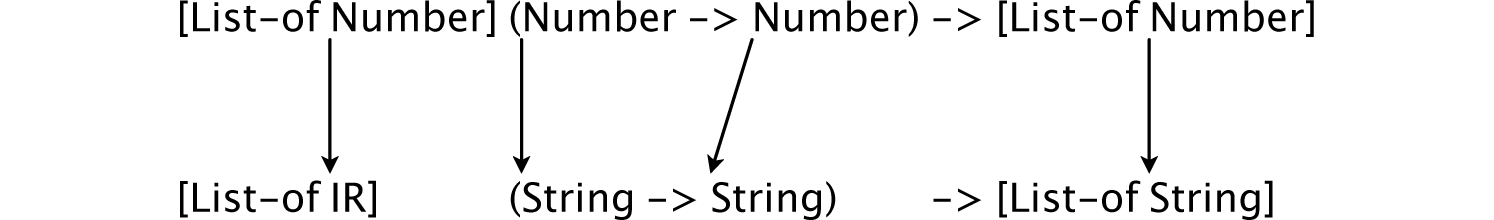
\includegraphics[width=0.85\textwidth]{images/00346.png}
\end{center}

连线标明了第二个参数（函数参数）内部的差异与原签名的差异紧密相关：新箭头左侧的 \code{Number} 与 \code{IR} 对应于首个列表参数中元素的类型；右侧的 \code{Number} 与 \code{String} 则对应于返回列表中元素的类型。

现在，我们应用同样的技巧，即可推导出 \code{map1} 的通用抽象签名：

\begin{lstlisting}[language=BSL]
; [X Y] [List-of X] [X -> Y] -> [List-of Y]
\end{lstlisting}

具体而言：\code{map1} 接收一个列表，其元素属于某种（尚待确定的）数据集合 \code{X}；它还接收一个能够将 \code{X} 类型的元素转换为另一类型 \code{Y} 的函数；最终，\code{map1} 产生一个包含 \code{Y} 类型元素的列表。

对签名进行抽象需要反复练习。让我们看第二个签名对：

\begin{lstlisting}[language=BSL]
; [List-of Number] -> Number
; [List-of Posn] -> Image
\end{lstlisting}

它们分别是练习 252 中 \code{product} 和 \code{image*} 的签名。结构对比表明：左侧签名中的第一个 \code{Number} 对应于右侧的 \code{Posn}，而第二个 \code{Number} 对应于右侧的 \code{Image}：

\begin{center}
  
\includegraphics[width=0.85\textwidth]{images/00347.png}
\end{center}

为了提炼出二者的抽象签名，我们遵循设计配方的前两个步骤：

\begin{stepperbox}
  \noindent\begin{minipage}[t]{0.48\linewidth}\vspace{0pt}
\begin{Verbatim}[commandchars=\\\{\}, fontsize=\fontsize{6.0pt}{7.2pt}\selectfont]
(define (pr* l bs jn)
  (cond
    [(empty? l) bs]
    [else
      (jn (first l)
          (pr* (rest l)
               bs
               jn))]))
\end{Verbatim}
  \end{minipage}\hfill
  \begin{minipage}[t]{0.48\linewidth}\vspace{0pt}
\begin{Verbatim}[commandchars=\\\{\}, fontsize=\fontsize{6.0pt}{7.2pt}\selectfont]
(define (im* l bs jn)
  (cond
    [(empty? l) bs]
    [else
      (jn (first l)
          (im* (rest l)
               bs
               jn))]))
\end{Verbatim}
  \end{minipage}
\end{stepperbox}

由于两个函数在两组值上存在差异，修改后的版本额外接收两个参数：一个是基础情形下的基本值，另一个是用于将自然递归的结果与给定列表的首项进行结合的函数。

为这两个新函数写出带有具体参数的签名：对于 \code{pr*}：
\begin{lstlisting}[language=BSL]
; [List-of Number] Number [Number Number -> Number] -> Number
\end{lstlisting}
因为基础情形产生一个数字，且组合函数是 \code{+}。对于 \code{im*}：
\begin{lstlisting}[language=BSL]
; [List-of Posn] Image [Posn Image -> Image] -> Image
\end{lstlisting}
因为基础情形返回一幅图像，组合函数是 \code{place-dot}（将一个 Posn 和一幅 Image 组合为新 Image）。

将两者的结构对比扩展到包含新增输入的完整签名中：

\begin{center}
  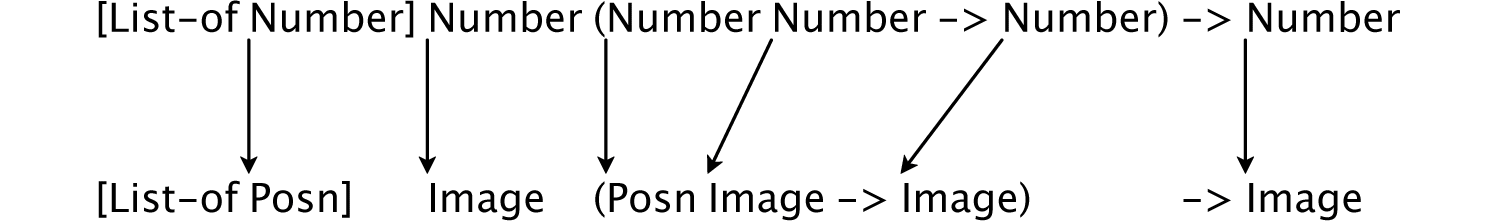
\includegraphics[width=0.85\textwidth]{images/00349.png}
\end{center}

这六对差异最终归结为两种本质对应：
\begin{enumerate}
  \item 部分 \code{Number} 对应于 \code{Posn}（由类型变量 \code{X} 表示）；
  \item 另一些 \code{Number} 对应于 \code{Image}（由类型变量 \code{Y} 表示）。
\end{enumerate}

由此，我们推导出了练习 252 中 \code{fold2} 抽象函数的普适签名：

\begin{lstlisting}[language=BSL]
; [X Y] [List-of X] Y [X Y -> Y] -> Y
\end{lstlisting}

\begin{notebox}[驻足验证类型实例化]
请务必停下来进行验证：将签名中的类型变量 \code{X} 与 \code{Y} 均替换为 \code{Number}，是否能够准确还原出 \code{pr*} 的签名？将它们分别替换为 \code{Posn} 和 \code{Image}，是否恰好得到 \code{im*} 的签名？
\end{notebox}

\begin{recipebox}{提炼抽象签名的系统步骤}
\begin{enumerate}
  \item \textbf{比较签名}：给定两个相似的函数定义 $f$ 与 $g$，对比它们的签名，标出相似的骨架与所有差异位置，并将相互对应的差异连线成对。
  \item \textbf{扩展签名}：为消除 $f$ 与 $g$ 的差异而引入抽象参数后，写出扩展后的中间签名。明确新增参数原本代表什么角色，以此确定新增参数的子签名。
  \item \textbf{引入类型参数}：检查步骤 1 中的对应分析是否依然适用于扩展签名。若适用，为每一类本质差异引入一个类型变量（如 \code{X}、\code{Y}）。当两个签名的表达式完全一致时，你就得到了通用的抽象签名。
  \item \textbf{检验与验证}：
    \begin{itemize}
      \item \textbf{代入检验}：通过对类型变量进行恰当的特化代入，必须能精确还原出各个具体函数的签名；
      \item \textbf{契约一致性}：检查通用签名与函数体代码是否完全吻合。若参数 $p$ 的签名为 \code{[A B -> C]}，则在代码中 $p$ 必须始终被传入两个参数（分别来自 $A$ 和 $B$），且调用 $p$ 的结果必须符合类型 $C$ 的上下文要求。
    \end{itemize}
\end{enumerate}
\end{recipebox}

\begin{exercise}{解读高阶函数签名}{253}
以下每个签名都描述了一类函数：
\begin{enumerate}
  \item \code{[Number -> Boolean]}
  \item \code{[Boolean String -> Boolean]}
  \item \code{[Number Number Number -> Number]}
  \item \code{[Number -> [List-of Number]]}
  \item \code{[[List-of Number] -> Boolean]}
\end{enumerate}
请用自然语言描述这些函数集合，并为每一类函数在 ISL 中给出至少一个具体的函数实例。
\end{exercise}

\begin{exercise}{排序函数的签名抽象}{254}
为以下两个函数分别拟定签名：
\begin{itemize}
  \item \code{sort-n}：接收一个数字列表和一个比较函数（该函数接收列表中的两个数字并返回布尔值），产生一个排好序的数字列表；
  \item \code{sort-s}：接收一个字符串列表和一个比较函数（该函数接收列表中的两个字符串并返回布尔值），产生一个排好序的字符串列表。
\end{itemize}
然后遵循上述配方对这两个签名进行抽象。并展示如何通过实例化该通用签名，来描述库存记录列表的排序函数 \code{sort-ir} 的签名。
\end{exercise}

\begin{exercise}{映射函数的签名抽象}{255}
为以下两个函数分别拟定签名：
\begin{itemize}
  \item \code{map-n}：接收一个数字列表和一个从数字到数字的函数，产生一个新的数字列表；
  \item \code{map-s}：接收一个字符串列表和一个从字符串到字符串的函数，产生一个新的字符串列表。
\end{itemize}
然后遵循上述步骤对这两个签名进行抽象。并展示如何将提炼出的通用签名实例化为前文 \code{map1} 函数的签名。
\end{exercise}

% ------------------------------------------------------------------------------
\section{单点控制原则}
\label{sec:15_3}

在广义上，编写程序就像撰写论文草稿。修改草稿对于纠正拼写错误、修饰语法漏洞、保持全书文风一致以及消除冗余重复至关重要。没有人愿意阅读充满大量重复段落的文章，更没有人愿意维护充斥着重复代码的软件系统。

消除代码中的相似性以提炼抽象具有不可估量的巨大优势：
\begin{itemize}
  \item 提炼抽象大幅简化了程序结构；
  \item 它能够暴露已有函数中潜藏的缺陷（尤其是当相似之处存在微妙偏差时）；
  \item \textbf{最为关键的优势在于：它为通用功能建立了统一的单点控制原则（Single Point of Control）}。
\end{itemize}

将某种功能的实现逻辑集中在单一位置，使得程序的长期维护变得轻而易举。当你发现一处缺陷时，只需修改一处代码即可彻底修复；当你需要让代码兼容新的数据形态时，只需在一个地方添加扩展；当你发现一种算法上的性能优化时，一次改动即可让系统中所有依赖该功能的地方同步受益。反之，如果你到处复制粘贴并微调代码，你就必须手动找到所有散落的副本逐一修改，否则旧错误将阴魂不散，或者只有某一个函数跑得飞快而其他地方依然缓慢。

\begin{notebox}[现代软件工程的核心准则]
\textbf{构建抽象，绝不复制粘贴并修改代码！} (Form an abstraction instead of copying and modifying any code.)
\end{notebox}

我们用于抽象函数的设计配方是构建抽象的最基础武器。掌握它需要大量的实战练习。随着熟练度的提升，你阅读、组织和维护复杂系统的能力将成倍跃升。最顶尖的程序员总是那些主动重构代码、积极提炼抽象、将相关逻辑收敛于单一控制源（单点控制原则）的工程师。在面向对象编程语言中，你还将接触到这一思想的另一种经典实现形态：基于类的继承与多态机制。

% ------------------------------------------------------------------------------
\section{从模板中提炼抽象}
\label{sec:15_4}

本部分的前两章展示了许多基于相同模板构建的函数。毕竟，设计配方的核心原则正是：\textbf{依据主要输入数据的组织结构来组织函数架构}。因此，处理同类数据的函数在外观与骨架上高度相近也就理所当然了。

事实上，我们甚至应当直接\textbf{对设计模板本身进行抽象}，而且这种抽象在理论上完全可以自动化完成（某些前沿的实验性编程语言已经做到了这一点）。尽管自动化推导仍是计算机科学的前沿研究课题，但你现在完全有能力理解其核心理念。

请观察我们熟悉的列表处理模板：

\begin{lstlisting}[language=BSL]
(define (fun-for-l l)
  (cond
    [(empty? l) ...]
    [else (... (first l) ...
               ... (fun-for-l (rest l)) ...)]))
\end{lstlisting}

该模板包含两个空白待填处，每个分支各有一个。当你利用此模板定义具体的列表处理函数时，你通常在第一个 \code{cond} 分支中填入一个具体的基准值，并在第二个分支中填入一个组合函数 \code{combine}。该 \code{combine} 函数接收列表的首项以及自然递归的结果，并将这两部分数据融合成最终的结果。

现在你已经掌握了如何创建抽象，完全可以从上述描述中直接定义出该模板的终极抽象函数——\code{reduce}：

\begin{lstlisting}[language=BSL, basicstyle=\scriptsize\ttfamily]
; [X Y] [List-of X] Y [X Y -> Y] -> Y
(define (reduce l base combine)
  (cond
    [(empty? l) base]
    [else (combine (first l)
                   (reduce (rest l) base combine))]))
\end{lstlisting}

它接收两个额外的实参：\code{base}（基准情形下的默认返回值）以及 \code{combine}（在第二分支中执行结果合并的二元函数）。

借助 \code{reduce}，你可以将绝大多数常规的列表处理函数直接写成优雅的“单行函数”。以下是求和 \code{sum} 与求积 \code{product} 的单行定义：

\begin{stepperbox}
  \noindent\begin{minipage}[t]{0.48\linewidth}\vspace{0pt}
\begin{Verbatim}[commandchars=\\\{\}, fontsize=\fontsize{6.0pt}{7.2pt}\selectfont]
; [List-of Number] -> Number
(define (sum lon)
  (reduce lon 0 +))
\end{Verbatim}
  \end{minipage}\hfill
  \begin{minipage}[t]{0.48\linewidth}\vspace{0pt}
\begin{Verbatim}[commandchars=\\\{\}, fontsize=\fontsize{6.0pt}{7.2pt}\selectfont]
; [List-of Number] -> Number
(define (product lon)
  (reduce lon 1 *))
\end{Verbatim}
  \end{minipage}
\end{stepperbox}

对于 \code{sum}，基础情形始终返回 0；而在第二分支中，通过 \code{+} 将首项与自然递归的结果相加。同样的推理完全解释了 \code{product}（基础情形返回 1，组合函数为 \code{*}）。几乎所有基础的列表处理函数，都可以通过这种方式用 \code{reduce} 简洁利落地定义出来！
